\documentclass[border=0mm]{standalone}
\usepackage{pgfplots}
\usepgfplotslibrary{groupplots}
\pgfplotsset{compat=1.17}
\usepackage{xcolor}
\usepackage{xstring}
\usepackage{ upgreek }
\usepackage{amsmath}



\definecolor{blue}{rgb}{0,0.4470,0.7410}
\definecolor{red}{rgb}{0.8500,0.3250,0.0980}

\begin{document}
\pgfplotsset{
compat=1.11,
legend image code/.code={
\draw[mark repeat=2,mark phase=2]
plot coordinates {
(0cm,0cm)
(0.15cm,0cm)        %% default is (0.3cm,0cm)
(0.3cm,0cm)         %% default is (0.6cm,0cm)
};
}
}%
\pgfdeclarelayer{background layer}%
\pgfdeclarelayer{foreground layer}%
\pgfsetlayers{background layer,main,foreground layer}%
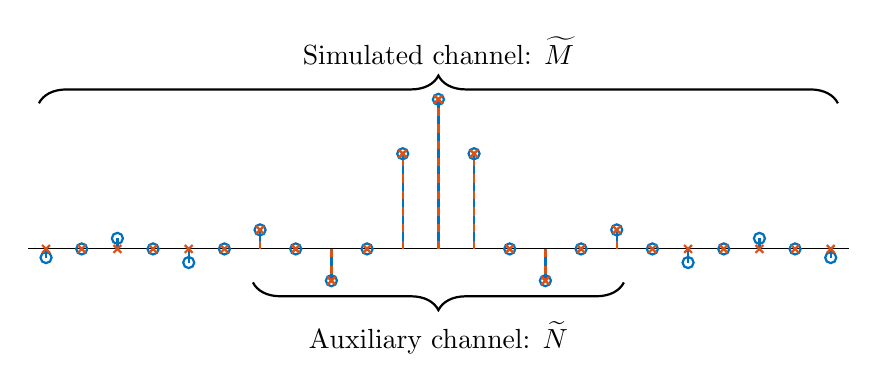
\begin{tikzpicture}[
declare function={
	sinc(\x) = (\x == 0) * 1+
			(\x!=0) * sin(pi*deg(\x))/(pi*\x) ;
},
>=stealth
]%
\begin{axis}[
  width = 12cm,
  height = 5cm,
  axis x line*=middle,  % Show only the x-axis
  axis y line=none,    % Hide the y-axis
  xmin=-5.75, xmax=5.75,
  ymin=-0.5, ymax=1.3,  % Set ymax to 2
  xtick=\empty,
  every tick label/.append style={scale=0.7},
  xlabel style={
    above,
  },
]%
\addplot [thick,ycomb, domain=-5.5:5.5, samples=23, blue, mark=o] {sinc(x)};
\addplot [dashed,thick,ycomb, domain=-2.5:2.5, samples=11, red, mark=x] {sinc(x)};
\addplot [thick,ycomb, domain=-2.5:2.5, samples=11, red, mark=x,only marks,] {sinc(x)};
\addplot [thick,ycomb, domain=-5.5:-3, samples=6, red, mark=x,only marks,] {0};
\addplot [thick,ycomb, domain=3:5.5, samples=6, red, mark=x,only marks,] {0};
\coordinate (p0) at (axis cs: -2.6,-0.15);%
\coordinate (p1) at (axis cs: 2.6,-0.15);%
\coordinate (p2) at (axis cs: -5.6,0.9);%
\coordinate (p3) at (axis cs: 5.6,0.9);%
\end{axis}%
\draw [thick,decorate,decoration={brace,amplitude=10pt,mirror,raise=4pt},yshift=0pt]
(p0) -- node [below,yshift=-0.5cm] {Auxiliary channel: $\widetilde{N}$}(p1);%
\draw [thick,decorate,decoration={brace,amplitude=10pt,raise=4pt},yshift=0pt]
(p2) -- node [above,yshift=0.5cm] {Simulated channel: $\widetilde{M}$}(p3);%
\end{tikzpicture}
\end{document}
























